\documentclass[a4paper]{article}
\usepackage[spanish]{babel}
\usepackage[utf8]{inputenc}
\usepackage{charter}   % tipografia
\usepackage{graphicx}
%\usepackage{makeidx}
\usepackage{paralist} %itemize inline

\usepackage{color} % para snipets de codigo coloreados
\usepackage{fancybox}  % para el sbox de los snipets de codigo

\definecolor{litegrey}{gray}{0.94}

% \newenvironment{sidebar}{%
% 	\begin{Sbox}\begin{minipage}{.85\textwidth}}%
% 	{\end{minipage}\end{Sbox}%
% 		\begin{center}\setlength{\fboxsep}{6pt}%
% 		\shadowbox{\TheSbox}\end{center}}
% \newenvironment{warning}{%
% 	\begin{Sbox}\begin{minipage}{.85\textwidth}\sffamily\lite\small\RaggedRight}%
% 	{\end{minipage}\end{Sbox}%
% 		\begin{center}\setlength{\fboxsep}{6pt}%
% 		\colorbox{litegrey}{\TheSbox}\end{center}}

\newenvironment{codesnippet}{%
	\begin{Sbox}\begin{minipage}{\textwidth}\sffamily\small}%
	{\end{minipage}\end{Sbox}%
		\begin{center}%
		\vspace{-0.4cm}\colorbox{litegrey}{\TheSbox}\end{center}\vspace{0.3cm}}




\usepackage{fancyhdr}

\pagestyle{fancy}

\renewcommand{\sectionmark}[1]{\markright{\thesection\ - #1}}

\fancyhf{}

\fancyhead[LO]{Sección \rightmark} % \thesection\ 
\fancyfoot[LO]{\small{Leandro Raffo, Maximiliano Fernández Wortman, Uriel Rozenberg.}}
\fancyfoot[RO]{\thepage}

\renewcommand{\headrulewidth}{0.5pt}
\renewcommand{\footrulewidth}{0.5pt}
\setlength{\hoffset}{-0.8in}
\setlength{\textwidth}{16cm}
%\setlength{\hoffset}{-1.1cm}
%\setlength{\textwidth}{16cm}
\setlength{\headsep}{0.5cm}
\setlength{\textheight}{25cm}
\setlength{\voffset}{-0.7in}
\setlength{\headwidth}{\textwidth}
\setlength{\headheight}{13.1pt}

\renewcommand{\baselinestretch}{1.1}  % line spacing




% \setcounter{secnumdepth}{2}

\usepackage{caratula}


\begin{document}


\thispagestyle{empty}
\materia{Organización del Computador II}
\submateria{Segundo Cuatrimestre de 2015}
\titulo{Trabajo Práctico II}
\subtitulo{Programacion SIMD}
\integrante{Leandro Raffo}{945/12}{leandrojavr@gmail.com}
\integrante{Maximiliano Fernández Wortman}{892/10}{maxifwortman@gmail.com}
\integrante{Uriel Rozenberg}{838/12}{urielrozenberg@hotmail.com}

%Pagina de titulo e indice
%\thispagestyle{empty}

\maketitle 

\tableofcontents

\newpage

\section{Introduccion}
En este trabajo práctico realizamos la implementación de dos filtros de imagenes, con tal de ver que tan eficiente puede llegar a ser (o no) SIMD, los filtros son la diferencia de imagenes y el blur gaussiano, los cuales fueron implementados en lenguaje C (gcc y clang) y assembly, haciendo uso de instrucciones vectoriales. Luego comparamos la performance de estas implementaciones sobre diferentes imagenes y usando herramientas probabilísticas y estadísticas.

\section{Implementacion}

\subsection{Diferencia}
\noindent Descripcíon de un ciclo de la iteración del filtro diferencia.\\
Primermo pedimos memoria para declarar las máscaras que vamos a usar y armamos el stackframe (omitido)
\begin{codesnippet}
\begin{verbatim}
section .rodata
mask_5 DB 2,2,2,2,6,6,6,6,10,10,10,10,14,14,14,14
trans_2 DB 0,0,0,255,0,0,0,255,0,0,0,255,0,0,0,255
\end{verbatim}
\end{codesnippet}

\noindent Luego de armar el stackframe tenemos
\begin{codesnippet}
\begin{verbatim}
mov r12, rdx
mov eax, r8d
mov ecx, ecx
mul rcx
xor r15, r15
\end{verbatim}
\end{codesnippet}
r12 apunta a la matriz resultado, ecx tiene la cantidad de filas, y la parte baja de rax tiene la cantidad de columnas. Al hacer mul rcx se tiene filas*columnas en rdx:rax, como las operaciones son de 32 bits tenemos la multiplicación en rax, que es lo que vamos a usar, junto a r15 para iterar. Ahora entramos al ciclo.

\begin{codesnippet}
\begin{verbatim}
.ciclo:
    cmp r15, rax
    JE .fin
\end{verbatim}
\end{codesnippet}

\noindent Comparamos si r15 es igual a rax en tal caso ya hicimos la diferencia sobre todos los pixeles y termina el ciclo. El ciclo sigue con

\begin{codesnippet}
\begin{verbatim}
    movdqu xmm3 , [RDI +  r15*4]   
    movdqu xmm15, [RSI +  r15*4]
    movdqu xmm14, xmm15     
    pminub xmm15, xmm3        
    pmaxub xmm3 , xmm14        
    psubb  xmm3 , xmm15             
    movdqu xmm4, xmm3 
    movdqu xmm5, xmm3       
\end{verbatim}
\end{codesnippet}

\noindent Movemos a xmm$3$ los primeros $4$ pixeles de la primera matriz y a xmm$15$ los primeros $4$ de la segunda matriz a comparar, estos ocupan respectivamente $16$ bytes en memoria (brga por $4$). Después Guardamos en xmm$14$ el valor de xmm$15$ y hacemos un pminub entre xmm$15$ y xmm$3$ lo cual deja en xmm$15$ el mínimo byte a byte. Lo mismo para xmm$3$ pero con pmaxub es decir este tiene el máximo byte a byte. Hacemos esto porque queremos calcular el valor absoluto de la forma $|x-y|$ = $\max(x,y) - \min(x,y)$. Concluimos esta idea haciendo psubb entre xmm$3$ que tenia el máximo y xmm$15$ que tenia el mínimo y finalmente guardamos el resultado en xmm$4,5$ para operar en la siguiente parte.

\begin{codesnippet}
\begin{verbatim}
    pslldq xmm4, 1                  
    pslldq xmm5, 2               
    movdqu xmm6, xmm5             
    pmaxub xmm6, xmm4             
    pmaxub xmm6, xmm3              
    pshufb xmm6, [mask_5] 
    paddsb xmm6, [trans_2]
    movdqu [r12 +  r15*4], xmm6
    add  r15d, 4
    jmp .ciclo
\end{verbatim}
\end{codesnippet}
\noindent Ahora shifteamos con packed shift xmm$4,5$ uno y dos bytes respectivamente de forma de poder tomar el máximo de entre r g b en paralelo, es decir $4$ pixels a la vez. Por ejemplo, el primer byte de xmm$4$ tiene al byte de r, y el de xmm$6$ tiene al byte de g, de forma que al hacer pmaxub entre  xmm$6$ y xmm$4$ nos deja en el primer byte de xmm$6$ (y cada 3 bytes) max(r$_n$,g$_n$) donde $n = \{1,2,3,4 \}$ indican los pixeles que levantamos. Los demas bytes de este registro no nos interesan. Repetimos esto entre xmm$6$ y xmm$3$, pasa de vuelta lo mismo pero ahora tenemos en el primer byte de xmm$6$ (y cada $3$ bytes) max(r$_n$,g$_n$,b$_n$) con $n = \{1,2,3,4 \}$. Ahora tenemos que mover este máximo a las 3 coordenadas r, g y b, hacemos esto mediante la mascara mask$_5$ y mediante trans$_2$ sumamos con saturación con tal de dejar en alpha el valor $255$. Copiamos los 16 bytes correspondientes (con el offset adecuado) en la matriz destino, sumamos $4$ a r$15$d y saltamos para, si es necesario, volver a hacer el ciclo completo.

\subsection{Blur gaussiano}

\noindent En el blur gaussiano calculamos 4 pixeles por iteración, pero para legibilidad solo vamos a escribir lo que le pasa a uno solo, se repite el código y se apunta a memoria correctamente. 

\begin{codesnippet}
\begin{verbatim}
movdqu xmm0,[r12]  
movdqu xmm1, xmm0
punpckhbw xmm0, xmm7 
punpcklbw xmm1, xmm7  
movdqu xmm2, xmm0
movdqu xmm3, xmm1
punpckhwd xmm0, xmm7  	
punpcklwd xmm2, xmm7   
punpckhwd xmm1, xmm7  
punpcklwd xmm3, xmm7  
\end{verbatim}
\end{codesnippet}

\noindent Primero levantamos $16$ bytes de memoria, equivalente a $4$ pixeles en xmm$0$ y lo copiamos en xmm$1$ ya que vamos a desempaquetar los datos. Llamamos a punpcklbw/hbw junto a un xmm$7$ que estaba en $0$, tenemos entonces que xmm$0$ tiene los primeros $2$ pixeles ($8$ bytes) extendidos a cada uno a un word. Lo mismo para xmm$1$. Luego repetimos el proceso desempaquetando a un double word, ya que queremos operar con floats y este es su tamaño. 

\begin{codesnippet}
\begin{verbatim}
cvtdq2ps xmm0,xmm0
\end{verbatim}
\end{codesnippet}



\newpage



\section{Resultados}

\subsection{Diferencia}

\noindent \textbf{Nota:} todos los tests fueron corridos sobre una PC con procesador Intel Core2Duo E8440.
\\
\noindent Para analizar las implementaciones de C y assembly, corrimos 1000 iteraciones de cada implementación de diferencia sobre una imagen de 2308x2308 (16mb) donde las implementaciones de C se compilaron con gcc y clang usando los flags de optimización -O0, -O1, -O2 y -O3.


\begin{figure}[h]
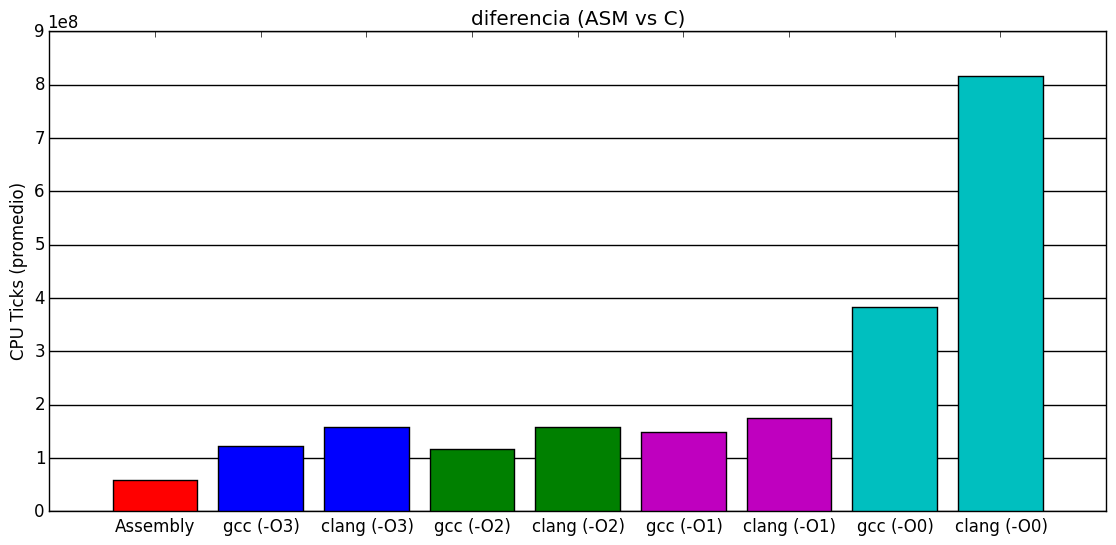
\includegraphics[scale=0.56]{imagenes/test_difrencia_ASM_C_promedio.png}
\caption{Promedio, sin outliers incluidos, sobre una imagen de 2308x2308 de 16mb.}
\end{figure}

\noindent Luego eliminamos los outliers y graficamos de vuelta obteniendo.\\


\begin{figure}[h]
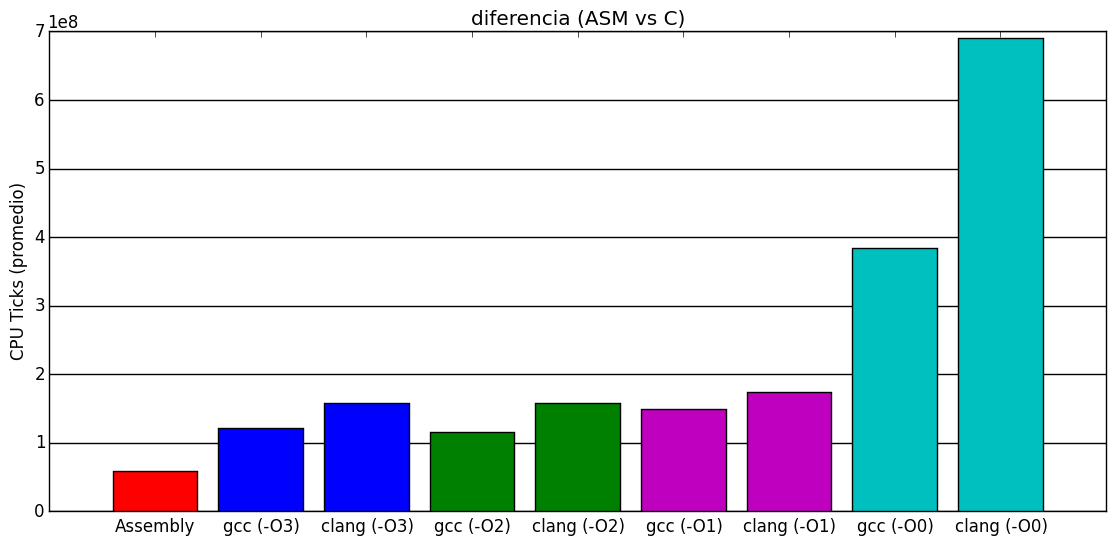
\includegraphics[scale=0.56]{imagenes/test_difrencia_ASM_C_no_outliers.png}
\caption{Promedio, con outliers incluidos, sobre una imagen de 2308x2308 de 16mb.}
\end{figure}

\noindent Vemos que clang en -O0 se comporta un poco mejor sacando esos resultados extremos, y lo que podemos concluir es que el algoritmo implementado en assembly con SIMD corre 2 veces más rapido que su contraparte en C.

\newpage 

\noindent En el siguiente experimento queria ver si el tamaño de la imagen iba a modificar la performance (incrementar el tiempo de ejecucion) del algoritmo debido a cache misses. Para esto corrimos diferencia en Assembly y C, de vuelta bajo gcc y clang, pero esta vez con el flag -O2, ya que me parecio que era el sweet spot para esta implementación ya que los flags de optimización no garantizan que corra con mejor performance, sobre imágenes que iban de 256kb a 64mb como se ve en la figura (Los tamaños utilizados están en el shellscript convertir.sh que es el que usamos para generar las imagenes). 

\begin{figure}[h]
	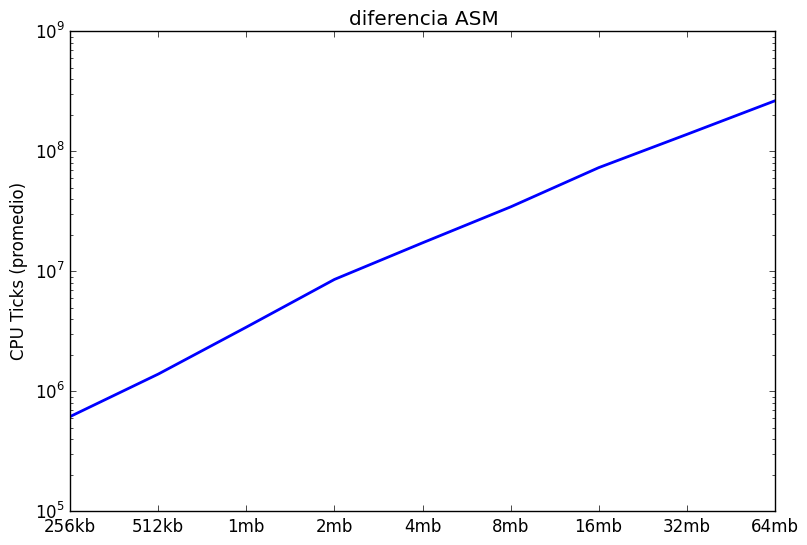
\includegraphics[scale=0.60]{imagenes/test_performance_size_ASM.png}
	\caption{Diferencia en asm, escala logarítmica}
\end{figure}

\noindent Lo que se obtuvo es una curva que sube suavemente, lo cual implicaria que el algoritmo tiene un crecimiento bastante predecible hasta el tamaño donde se lo probó (imágenes de 4000x4000 pixels con un tamaño de 64mb).

\begin{figure}[h]
	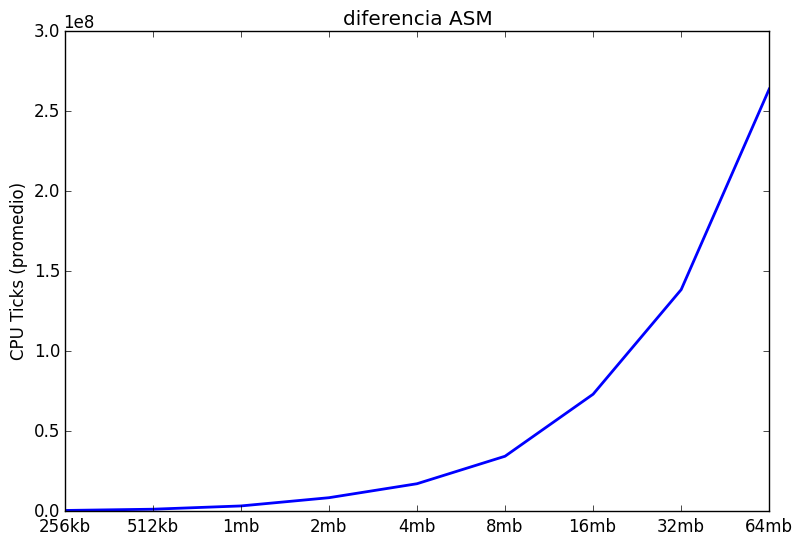
\includegraphics[scale=0.60]{imagenes/test_performance_size_ASM_not_log.png}
	\caption{Diferencia en asm, escala no logarítmica}
\end{figure}

\newpage 

Lo mismo pasa con las implementaciones en C, en este caso gcc con -O2.

\begin{figure}[h]
	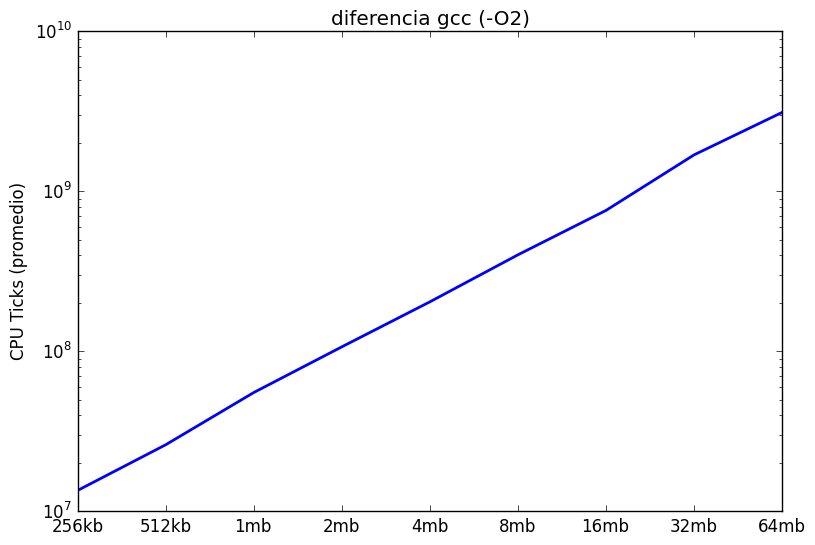
\includegraphics[scale=0.60]{imagenes/test_performance_size_C.png}
	\caption{Diferencia en C, escala logarítmica}
\end{figure}


\subsection{Blur}

\noindent Una de las hipótesis que teniamos con blur es que dada una imagen con un radio pequeño iba a correr mas lento que con un radio mas grande, pero a medida que el radio domine la cantidad de pixeles sobre las cuales va a aplicar la matriz de convolución el tiempo de ejecución iba a bajar. Esto lo pudimos probar corriendo blur sobre una imagen de tamaño fijo (en este caso 584x584 pixels) e incrementando el radio como se ve en la siguiente imagen

\begin{figure}[h]
	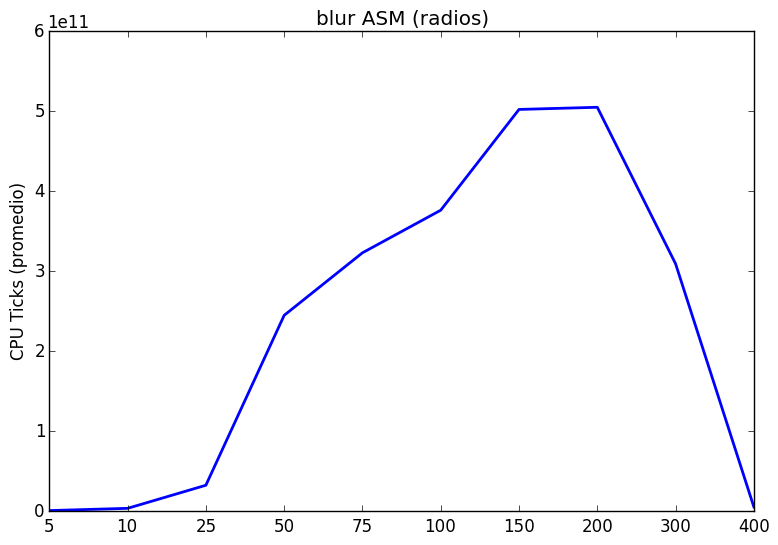
\includegraphics[scale=0.62]{imagenes/test_radio_size_ASM.png}
	\caption{Blur, cambiando los radios}
\end{figure}

El algoritmo llega a un punto crítico cuando el radio es equivalente a la dimensión/2, es decir cuando el algoritmo se comporta como $O(n^4)$ sobre la dimensión.


\newpage 

Para comparar al algoritmo en C vs asm hicimos lo mismo que blur, corrimos los dos sobre la misma imagen y calculamos su promedio.


\begin{center}
    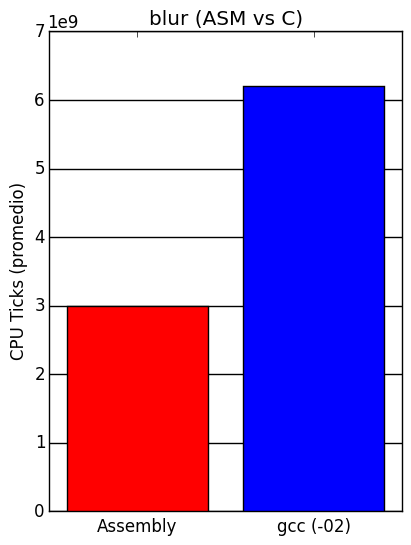
\includegraphics[scale=0.6]{imagenes/test_blur_ASM_C.png}
\end{center}

\section{Conclusión}

\noindent Para el algoritmo de diferencia, se justificaria totalmente hacer una implementación en SIMD, no solo por el hecho de que corre mas rápido, sino que además implementarlo en assembly fue bastante fácil ($<$ 20 lineas). Pasa lo contrario con blur, donde la performance ganada no es justificable contra el costo de implementarlo.

\end{document}
